\documentclass[11pt,letterpaper,]{paper}

\NeedsTeXFormat{LaTeX2e} 

\usepackage{etoolbox} % Required for conditional logic and easily changing commands

\newtoggle{unnumberedsections} % Create toggle for a class option
\settoggle{unnumberedsections}{false} % Default value for the class option
\DeclareOption{unnumberedsections}{\settoggle{unnumberedsections}{true}} % Set the class option toggle if the class option was used in the template

% \DeclareOption*{\PassOptionsToClass{\CurrentOption}{article}} % Pass through any extra options specified to the base class
\ProcessOptions\relax % Process class options

% \LoadClass[twocolumn]{article} % Load the base class

%----------------------------------------------------------------------------------------
%	REQUIRED PACKAGES AND MISC CONFIGURATIONS
%----------------------------------------------------------------------------------------
 
\usepackage[bottom, hang]{footmisc} % Force footnotes to the bottom of the page and to the left margin
\setlength{\footnotemargin}{6pt} % Horizontal space between the footnote marker and text

%----------------------------------------------------------------------------------------
%	MARGINS
%----------------------------------------------------------------------------------------

\usepackage[
	top=2.5cm, % Top margin
	bottom=2.5cm, % Bottom margin
	left=2.2cm, % Left margin
	right=2.2cm, % Right margin
	footskip=1cm, % Space from the bottom margin to the baseline of the footer
	headsep=0.75cm, % Space from the top margin to the baseline of the header
	columnsep=20pt, % Space between text columns (in twocolumn mode)
	%showframe % Uncomment to show frames around the margins for debugging purposes
]{geometry}

%----------------------------------------------------------------------------------------
%	FONTS
%----------------------------------------------------------------------------------------

\usepackage[utf8]{inputenc} % Required for inputting international characters
\usepackage[T1]{fontenc} % Output font encoding for international characters

% \usepackage[sc]{mathpazo} % Use the Palatino font

\linespread{1.05} % Increase line spacing slightly

% \usepackage{microtype} % Slightly tweak font spacing for aesthetics

%----------------------------------------------------------------------------------------
%	HEADERS AND FOOTERS
%----------------------------------------------------------------------------------------

\usepackage{fancyhdr} % Required for customizing headers and footers
\pagestyle{fancy} % Enable custom headers and footers

\renewcommand{\headrulewidth}{0pt} % Top horizontal rule thickness

% \fancyhf{} % Clear default headers/footers

\fancyhead[L]{\small\textit{Choi 2023 Onsager} }  
% \fancyhead[L]{\small\textit{Choi 2023 Onsager} % Left-even page header

\fancyfoot[L]{\footnotesize{} }
% \fancyfoot[RO]{\small\textbf{\thepage}} % Right-odd page footer
% \fancyfoot[LO]{\footnotesize\} % Left-odd page footer
% \fancyfoot[LE]{\small\textbf{\thepage}} % Left-even page footer
% \fancyfoot[RE]{\footnotesize\} % Left-even page footer
 
 
%----------------------------------------------------------------------------------------
%	SECTIONS
%----------------------------------------------------------------------------------------

\usepackage{titlesec} % Required for modifying sections

\iftoggle{unnumberedsections}{ % Conditional logic for the unnumbered sections class options
	\setcounter{secnumdepth}{0} % Don't number sections at any level
}{
	\setcounter{secnumdepth}{2} % Number sections down to subsections
}

\titleformat
	{\section} % Section type being modified
	[block] % Section layout type, can be: hang, block, display, runin, leftmargin, rightmargin, drop, wrap, frame
	{\Large\bfseries\centering} % Text formatting of the whole section, i.e. label and title
	{\thesection} % Section label (e.g. number) and its formatting
	{0.5em} % Horizontal space between the section label and title
	{} % Code before the section title
	[] % Code after the section title

%------------------------------------------------

\titleformat
	{\subsection} % Section type being modified
	[block] % Section layout type, can be: hang, block, display, runin, leftmargin, rightmargin, drop, wrap, frame
	{\raggedright\large\bfseries} % Text formatting of the whole section, i.e. label and title
	{\thesubsection} % Section label (e.g. number) and its formatting
	{0.5em} % Horizontal space between the section label and title
	{} % Code before the section title
	[] % Code after the section title

%------------------------------------------------

\titleformat
	{\subsubsection} % Section type being modified
	[runin] % Section layout type, can be: hang, block, display, runin, leftmargin, rightmargin, drop, wrap, frame
	{\bfseries} % Text formatting of the whole section, i.e. label and title
	{} % Section label (e.g. number) and its formatting
	{5pt} % Horizontal space between the section label and title
	{} % Code before the section title
	[] % Code after the section title

\titlespacing*{\subsubsection}{0pt}{0.5\baselineskip}{8pt} % Spacing around section titles, the order is: left, before and after

%----------------------------------------------------------------------------------------
%	TITLE SECTION CUSTOMIZATION
%----------------------------------------------------------------------------------------

\usepackage{titling} % Required for customizing the title section

\setlength{\droptitle}{-4\baselineskip} % Move the title up

\pretitle{\begin{center}\huge\bfseries} % Article title pre-formatting
\posttitle{\end{center}} % Article title post-formatting

\setlength{\thanksmarkwidth}{3pt} % Left margin for the first \thanks line
\setlength{\thanksmargin}{-3pt} % Left margin for the second and onwards \thanks line

\patchcmd{\maketitle}{plain}{empty}{}{} % Set the headers and footers style for the first page to empty

%----------------------------------------------------------------------------------------
%	ABSTRACT CUSTOMIZATION
%----------------------------------------------------------------------------------------

\usepackage{abstract} % Allows abstract customization

\renewcommand{\abstractnamefont}{\normalfont\bfseries\vspace{0.5\baselineskip}} % Set the "Abstract" text to bold
\renewcommand{\abstracttextfont}{\vspace{-0.5\baselineskip}\normalfont\small\itshape} % Set the abstract itself to small italic text
 
%----------------------------------------------------------------------------------------
%	TABLES
%----------------------------------------------------------------------------------------

\usepackage{booktabs} % Required for better horizontal rules in tables

\usepackage{array} % Required for manipulating table columns

\newcolumntype{R}[1]{>{\raggedleft\arraybackslash}p{#1}} % Define a new right-aligned paragraph column type
\newcolumntype{L}[1]{>{\raggedright\arraybackslash}p{#1}} % Define a new left-aligned (no justification) paragraph column type
\newcolumntype{C}[1]{>{\centering\arraybackslash}p{#1}} % Define a new centered paragraph column type

%----------------------------------------------------------------------------------------
%	CAPTIONS
%----------------------------------------------------------------------------------------

\usepackage{caption} % Required for customizing captions

\captionsetup{skip=6pt} % Vertical whitespace between figures/tables and the caption (default is 10pt)
\captionsetup{labelfont={bf,small}, textfont={it,small}} % Define caption font style

%----------------------------------------------------------------------------------------
%	LISTS
%----------------------------------------------------------------------------------------

\usepackage{enumitem} % Required for list customization

\setlist{noitemsep} % Customize spacing around and inside lists

%----------------------------------------------------------------------------------------
%	LINKS
%----------------------------------------------------------------------------------------

\usepackage{hyperref} % Required for links

\hypersetup{
	colorlinks=true, % Whether to color the text of links
	urlcolor=black, % Color for \url and \href links
	linkcolor=black, % Color for \nameref links
	citecolor=black, % Color of reference citations
}

%----------------------------------------------------------------------------------------
%	CUSTOM COMMANDS
%----------------------------------------------------------------------------------------


\usepackage{ifxetex,ifluatex}

\usepackage{lmodern}

\IfFileExists{microtype.sty}{\usepackage{microtype}}{}

%% The amssymb package provides various useful mathematical symbols
\usepackage{amssymb}
%% The amsthm package provides extended theorem environments
%% \usepackage{amsthm}
\usepackage{amsmath}

%% The lineno packages adds line numbers. Start line numbering with
%% \begin{linenumbers}, end it with \end{linenumbers}. Or switch it on
%% for the whole article with \linenumbers after \end{frontmatter}.





\usepackage[authordate, maxcitenames=1, uniquename=mininit, backend=biber, natbib]{biblatex-chicago}
% \usepackage[]{biblatex}
% \usepackage[backend=biber, style=]{biblatex}
\addbibresource{references.bib}


\providecommand{\tightlist}{%
  \setlength{\itemsep}{0pt}\setlength{\parskip}{0pt}}

\setcounter{page}{1} % The page number of the first page, set this to a higher number if the article is to be part of an issue or larger work

 

\setlength{\parindent}{0pt}
\setlength{\parskip}{6pt plus 2pt minus 1pt}
\setlength{\emergencystretch}{3em}  % prevent overfull lines




  
\usepackage{authblk}
 
\author[ ]{Jae S. Choi and Roger I.C. Hansell}


%%------------/AUTHORS--------------


% % Affiliations are output in the \date{} command
% \date{\footnotesize\textsuperscript{\textbf{1}}School of Chemistry, The University of Michigan\\ \textsuperscript{\textbf{2}}Physics Department, The University of Wisconsin\\ \textsuperscript{\textbf{3}}Biological Sciences Department, The University of Minnesota}
\date{\today}

% Full-width abstract
\renewcommand{\maketitlehookd}{%
	\begin{abstract}
		\noindent There are two complementary approaches to thermodynamics, one
is an empirical, phenomenological representation of macroscopic states
and the second is a model-based, statistical-mechanical representation
of microscopic states. If only a few energy transformation steps are
involved, macroscopic quantities such as energy and entropy can be
estimated without ambiguity, and often the associated microscopic states
are well characterised. Both approaches have been used to develop and
guide many key early ecological ideas. However, most ecosystems are
characterized by uncountably many transformations that operate on a wide
range of space and time scales. This renders the bounds of such systems
ambiguous making both the macroscopic and microscopic approaches a
challenge. As such, the implementation of both approaches remain areas
ripe for further investigation. In particular, the Onsager reciprocal
relations permit simplification of expectations that are yet to be fully
understood in an ecological context. Here we begin to take a few first
steps in trying to understand the far-reaching ramifications of these
thermodynamic relations.
	\end{abstract}
}


\usepackage{graphicx}
\setkeys{Gin}{keepaspectratio}
% Scale images if necessary, so that they will not overflow the page
% margins by default, and it is still possible to overwrite the defaults
% using explicit options in \includegraphics[width, height, ...]{}
%\setkeys{Gin}{width=\maxwidth,height=\maxheight,keepaspectratio}

% Redefine \includegraphics so that, unless explicit options are
% given, the image width will not exceed the width of the page.
% Images get their normal width if they fit onto the page, but
% are scaled down if they would overflow the margins.
\makeatletter
\def\ScaleIfNeeded{%
  \ifdim\Gin@nat@width>\linewidth
    \linewidth
  \else
    \Gin@nat@width
  \fi
}
\makeatother
\let\Oldincludegraphics\includegraphics
{%
 \catcode`\@=11\relax%
 \gdef\includegraphics{\@ifnextchar[{\Oldincludegraphics}{\Oldincludegraphics[width=\ScaleIfNeeded]}}%
}%

 
 

%----------------------------------------------------------------------------------------
%	TITLE SECTION
%----------------------------------------------------------------------------------------

\title{Onsager's relations and Ecology}


%----------------------------------------------------------------------------------------

\begin{document}

\maketitle % Output the title section


Keywords - Order, Disorder, Entropy, Dissipative structures,
Nonequilibrium Thermodynamics, Le Chatelier-Braun Principle, Onsager's
Reciprocal Relations, Least Specific Energy Dissipation Principle


 
  
%% main text
\section[Introduction]{\texorpdfstring{Introduction\footnote{This paper
  is written for ecologists that aim to understand the intersection
  between Thermodynamics, especially in the tradition developed by
  Onsager, with Ecology. Current science in general and ecology and
  inter-disciplinary-thermodynamics in particular exists on a trajectory
  with little coherence and many cliques. This paper is written for the
  few that that will one day embark on this difficult journey littered
  with many paths, often poorly marked and meandering. Though there is
  nothing wrong with walking on meandering paths, I hope this helps to
  mark out the main guide posts to make your journey a little more
  coherent.}}{Introduction}}\label{introduction1}

A coherent understanding of empirically observed \emph{thermodynamic}
states of matter was developed by Carnot (1824), Thompson (1849) and
Clausius (1850). It was a monumental feat in that only a few variables
of state (temperature, pressure, volume) were sufficient to describe the
behavior of matter even if they were composed of an enormous number of
atoms and molecules. Shortly thereafter, Boltzmann (1877) and Gibbs
(1902) developed a statistical-mechanical description of the component
parts that was complementary and related to the former by a
proportionality factor (Boltzmann's constant; Planck 1901).

All ecological processes are subject to these same thermodynamic
laws\footnote{Landsberg's (1961, 1972) representation of the laws of
  thermodynamics are amongst the most concise and clear as they are
  simple postulates of existence:

  \begin{itemize}
  \tightlist
  \item
    \(0^\text{th}\) law: empirical temperature exists.
  \item
    \(1^\text{st}\) law: internal energy exists. Energy is conserved; it
    is not created nor destroyed, only transformed.
  \item
    \(2^\text{nd}\) law: \emph{entropy} and absolute temperature exists.
    Every energy transformation results in some form of unrecoverable
    loss, \emph{entropy}.
  \item
    \(3^\text{rd}\) law: systems cannot attain a temperature of 0
    Kelvin.
  \item
    \(4^\text{th}\) law: \emph{extensive} (aggregate) and
    \emph{intensive} (density) variables exists, for equilibrium states
    and at least some subset of near-equilibrium/non-equilibrium states.
  \end{itemize}}. Even the most basic attempts to account or model
matter and energy flows necessarily begin by invoking conservation of
energy and matter, and as such, irreversible losses of energy from the
system. There have been many attempts to understand this connection and
draw inferences from it, due to the possibility of similarly and
dramatically reducing the very large degrees of freedom required to
describe ecological systems into a few variables of ecological
``state'', and perhaps, even understanding the directionality of
ecological dynamics.

Unfortunately, most ecological systems exhibit matter and energy cycling
and boundary flows that occur at many space and time scales. This makes
accounting for \emph{entropy} very difficult/impossible (Meysman and
Bruers 2010). As such, many resort to a model-based,
information-theoretic representations of microscopic variability as an
analogue to microscopic \emph{disorder}. Further, due to the rather
spectacular successes of Boltzmann (1877), most authors conflate the two
concepts of macroscopic entropy and microscopic disorder. Indeed, it is
only when both the microscopic and the macroscopic descriptions of a
given system in focus can be shown to converge that we can begin to
suggest that we reasonably understand the system. In molecular motion,
certainly this connection has been demonstrated and so we say we
``understand'' it. But in ecological systems, both microscopic and
macroscopic representations are far from convergent. It is, therefore,
necessary to keep these two streams separate as they carry different
perspectives and we need to be cognizant of, how much, or how little,
they converge, such that we can gauge how well we ``understand'' an
ecological system.

Here we review some of the key issues related to the application of
thermodynamics in the field of ecology (see also: Fath et al.~2004,
Chakrabarti and Ghosh 2009, Meysman and Bruers 2010, Yen et al.~2014,
Choi 2019). In particular, we touch upon the conceptual beauty and
challenges of information theoretic Order Principles; the macroscopic,
\emph{extrinsic} focus of free energy gradient dissipation approaches
and with similar limitations; and finally upon Onsager's (1931a,b)
far-reaching contributions to connect the two: microscopic with the
macroscopic, which has still not yet been sufficiently appreciated by
ecologists, even after almost a hundred years since their expression.

\section{Microscopic Order}\label{microscopic-order}

Boltzmann (1877) connected the logarithm of the number of possible
configurations of microscopic states in the phase space
(statistical-mechanical) representation of a system to its macroscopic
state variable, \emph{entropy}, through a proportionality factor.
Boltzmann (1877) and subsequently, Gibbs (1902) suggested that this
increase in the number of microscopic states in phase space represents
the amount of randomness or variability in potential microscopic states.
The canonical example is an isolated container filled with \emph{n}
molecules of some gas, identical in all respects including, velocity and
momentum. As it would take much energy and effort to force the molecules
to stay in such a \emph{uniform} state, the potential energy can be
considered high and the \emph{entropy} associated with this
configuration can be considered to be at some reference value. As it has
only one microscopic state in the 6\emph{n}-dimensional phase space (2
variables of state \(\times\) 3 dimensions \(\times\) \emph{n}
molecules), the microscopic variability of the system can also be
considered low. Releasing the constraints that forced it to stay in this
state, the potential energy is eventually converted into kinetic energy
and residual \emph{entropy}. The latter quantity continues to increase
relative to the reference entropy state, as by definition it is
irreversible. Simultaneously, the movements and collisions of the gas
molecules will result in a spread of the velocity and momentum
distributions with each collision until eventually this distribution no
longer changes. The number of possible microscopic representations in
phase space increases to a maximum level of randomness or microscopic
(\emph{order \(\rightarrow\) disorder}) with a corresponding increase in
macroscopic \emph{entropy}. Basic elementary grade physics.

Similarly, an internal combustion engine takes the chemical potential
energy of fuel and in the process of burning it, converts it into
dispersed gases, small particulates and heat, some fraction of which
becomes \emph{entropy}. From a microscopic perspective: the
physical-chemical model of long-chained hydrocarbons and associated bond
energies, the fuel goes from a structured to a dis-aggregated state;
that is, the number of possible microscopic states in phase space has
increased (\emph{order \(\rightarrow\) disorder}).

Schrödinger (1944) pointed out that biological systems seem to operate
in a different manner. The example he used was DNA, which he described
as a curious ``aperiodic crystal'' of extremely high information
content, that is, with all the information required to create and
maintain life. He noted that DNA manages to replicate itself with
extreme stability as mutation rates are much lower than might be
expected simply due to thermal replacement and degradation in chemical
reaction of similarly large molecules. If DNA is represented as a phase
space with dimensionality equal to the number of base pairs; this
implies a model that assumes each base pair acts independently, which is
of course incorrect. But nonetheless, with each replication from parent
to child the amount of order remains roughly constant and the range of
variability at each base pair constrained to be within a range not too
dissimilar from the previous generation. Thus, the range of possible
microscopic states are narrow, stable and robust, suggesting an
\emph{order \(\rightarrow\) order} process.

This stability is due to chemical activation energies and chemical bond
stability; self-correcting enzyme systems and proteins; and of course
Darwinian selection. Indeed, stable life cycles, developmental
processes, canalization, phenotypic plasticity, ordered metabolic
pathways such as the Krebs cycle, predator-prey interactions,
host-parasite interactions, habitat-niche considerations, animal
migration patterns, species distributions in space, all represent
examples of intricately patterned or constrained processes of
\emph{order \(\rightarrow\) order}. They are the mainstay of biology and
ecology: feedback cycles and their inter-relationships (Yodzis 1981,
1988). More generally, such structures are also known as
\emph{dissipative structures} (Kolmogorov 1941, Glansdorff and Prigogine
1974); they describe these stable, \emph{order \(\rightarrow\) order}
systems that maintain their internal (local) structure/order, at the
cost of elevated energy degradation to their environment. In other
words, if the focus includes these structure and its surrounding
environment, then the overall effect is \emph{(local order \(<=>\) local
order) \(\rightarrow\) (global disorder)}, literally pumping free energy
in and entropy out. Other examples of this have been identified
including: Rayleigh-Bénard convection cells, the Zhabotinsky reactions
and Turing waves (Glansdorff and Prigogine 1974). Living systems, in the
act of growth and maintenance, tap into these external matter and energy
flows to maintain local order (Zotin and Zotina 1967).

Schrödinger (1944) also considered the steps that might be required to
lead to the origin of life, from simple chemical compounds to more
complex matter/energy cycles or ``hypercycles'' and eventually the
evolution of replication mechanisms such as RNA, DNA, proteins and
membrane based compartmentalization in the backdrop of strong energy
gradients (Eigen and Schuster 1979; Wicken 1980). They clearly suggest
the operation of yet another principle, \emph{disorder \(\rightarrow\)
order} and much has been said on this topic (Lotka 1922, Schrödinger
1944, Bertalanffy 1950, Eigen and Schuster 1979, Wicken 1980, Wiley and
Brooks 1982, Schneider and Kay 1994, Schneider and Sagan 2005, England
2013). In general, they suggest that living systems seem to increase in
complexity over evolutionary time: the sheer number, types and
hierarchical organization of structures and metabolic pathways is high
relative to our primordial ancestors that were presumably much simpler
and had shorter snippets of (D/R)NA, and in terms of the metabolic and
organizational structures that they encoded. With this increase in
complexity, there is seemingly a corresponding increase in \emph{order}
in the biota, due to the additional effort required to maintain this
complex and often intricate biological structure. In other words, the
action of Darwinian selection in the short-term seems to be to stabilize
(\emph{order \(\rightarrow\) order}) and in the long-term to increase
order (\emph{disorder \(\rightarrow\) order}); where the latter occurs
presumably through the accumulation of strategies for survival in the
face of a relentlessly variable abiotic and biotic environment (van
Valen 1976, Bell 1982).

This potential incongruence of \emph{(dis)order \(\rightarrow\) order}
with the \(2^\text{nd}\) law expectation of ever increasing
\emph{entropy} (and \emph{order \(\rightarrow\) disorder}) has even been
suggested by many of the above authors as being a means of defining or
distinguishing between life and nonlife. Indeed, Lovelock (1972),
Lovelock and Margulis (1974) used this logic to advantage and suggested
the ``Gaia hypothesis'', that the presence of atmospheric homeostasis
(i.e., a non-equilibrium stable state) can be used as an indicator of
the presence of life on other planets and is now even used as an
organizing principle of planetary-scale atmospheric models (Kleidon
2010). Similar kinds of thermodynamic inference have been made for
ecological succession, the stage-like patterns of colonization and
abundance in various landscapes and increase in order over ecological
time scales (Odum and Pinkerton 1955, MacArthur and Pianka 1966, E.P.
Odum 1969, Margalef 1963, Gladyshev 1978, Matsuno 1978, Johnson 1981,
Vanriel and Johnson 1995, Washida 1995, Kay 1991) and embryonic and
developmental patterns (Zotin and Zotina 1967, Lurié and Wagensberg
1979, Briedis and Seagrave 1984, Aoki 1989, Holdaway et al.~2010).

The presence of these three order principles has precipitated a wide,
generally confusing discussion of their relevance in living systems.
What has been learned through these discussions is that it is absolutely
necessary to specify explicitly the frames of reference by which we
mean: (1) the focal perspective (microscopic order/disorder or
macroscopic energy/matter); (2) the constraints such as boundary
conditions, ground/reference states; and (3) the space-time scales.

~

\begin{figure}
\centering
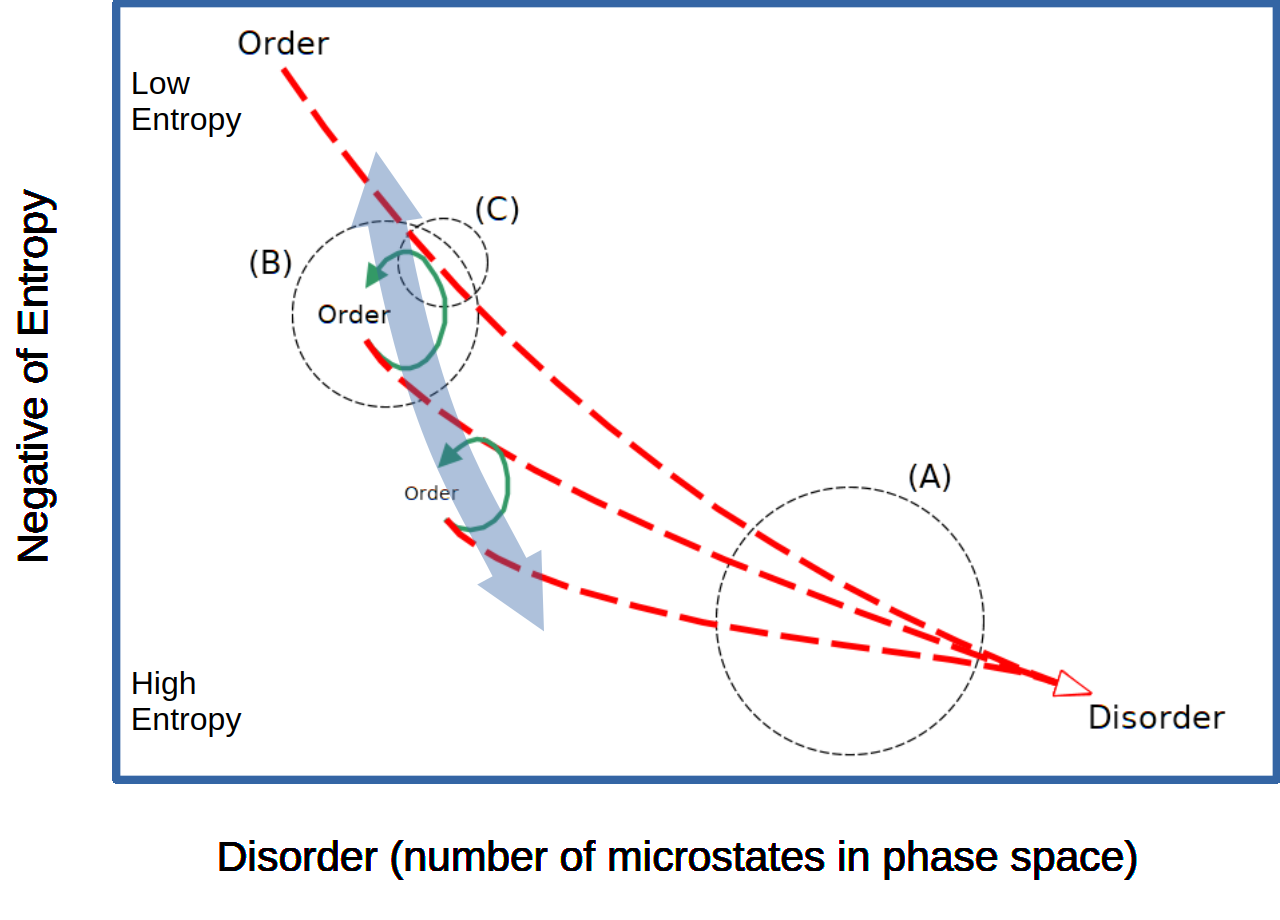
\includegraphics[width=0.8\textwidth,height=\textheight]{media/order_cascade.png}
\caption{Heuristic representation of the principles of order principles
and corresponding changes in entropy. (A) \emph{order \(\rightarrow\)
disorder}: the \(2^\text{nd}\) law such as in simple heat engines (red
dashed lines); (B) \emph{order \(\rightarrow\) order}: a seeming stasis,
that is, homeostatic behavior in biochemical systems, stable ecological
systems, genetic stability (green self-loop, and ``dissipative
structures''); and (C) \emph{disorder \(\rightarrow\) order}: a seeming
reversal of the \(2^\text{nd}\) law, observed in embryogenesis,
succession, biodiversity increase over evolutionary time scales
(transition from red-dashed lines to green loops). The circles show the
focal (local) processes for each order principle. Note the
dissipation-cascade from top to bottom as each dissipative structure
connects to other dissipative structures and manifested as Onsager
Relations (blue arrows; see text below), interconnected vehicles of
energy-cascades (turbulent dynamics, food-web dynamics, metabolic
pathways, etc.). Adapted from Choi (2019). \label{fig_cascade}}
\end{figure}

~

To illustrate the above, we use the simple metaphor of a parcel of water
flowing downhill along multiple paths/streams (Fig. \ref{fig_cascade},
area A). The potential energy of the parcel of water, a certain volume
tagged in the middle of a lake, at elevation is initially in a low
kinetic energy and high potential energy configuration, and being
otherwise in a similar state (pressure, volume, temperature), at some
initial level of entropy. As some of it flows down hill, some of the
potential energy is converted into kinetic energy and some dissipated as
heat, noise, erosion, percolation into groundwater, evaporation and
ultimately entropy. Given enough time, it will eventually reach the
lowest elevation possible (the equilibrium ``reference'' state in this
example), where it is in the highest possible \emph{entropy} state in
that all potential energy has been converted to entropy or kinetic
molecular energy. Simultaneously, the \emph{order} in the initial state
(low and uniform molecular momentum and velocity of the initial parcel
of water) when exposed to different pathways (streams, groundwater,
evaporation) progressively takes on increasingly more variable
distributions of momentum and velocity: spread out through the
atmosphere, in the lake, rivers, falls, in the ground, and the ocean
(\emph{disorder}) until it reaches the final highest disordered
reference state (the definition of which, depends upon the available
free energy entering the system).

However, under certain circumstances and space-time scales of
observation, the flow of water might seem to persist and gather
together, for a short period, such as for example, in eddies and pools
near rapids and falls. In the frame of these smaller windows (scales) of
time and space, these cycling structures can seem stable and
self-perpetuating: that is \emph{order \(\rightarrow\) order} (Fig.
\ref{fig_cascade}, area (B)). Though of course, it is only a small
volume that becomes part of the eddy and the bulk of the water continues
to flow downhill. And so the question is: what are these special
``certain circumstances''? As biologists and ecologists we endeavor to
detail all these special ``certain circumstances'' and pre-conditions to
stable material and energy flows, be they at subcellular, cellular,
organismal, population, community, ecosystem or earth-system levels of
organization.

In ecology, there is an \emph{implicit} understanding that these matter
and energy flows are only borrowed by biota, taking in a small fraction
of energy and matter (ecological efficiencies tend to be low relative to
``bulk flow'', see below) and so slowing down its eventual passage by
redirecting them into organisms and ecosystems by growth and
reproduction (biomass, chemical bonds), before their final release back
into the entropic flow, ``down the river'' in the form heat, noise,
breaking of molecular bonds, etc. Biota and ecological structures are
like these eddies and energy cascades. Indeed, this is so implicit that
seldom are the entropic flows and constraints the explicit focus in
biological and ecological studies. There is a matter-of-fact,
\emph{apriori} awareness that they are systems open to energy and matter
flows, where boundary inflows must be much larger than the outflows to
sustain life. Instead, ecologists tend to focus preferentially upon the
more ``interesting'' features of stable interactions and negative
feedback dynamics in the 1 to 10\% that is used or retained by biota.

Nonetheless, these more ``interesting'' eddy-like matter/energy
interactions facilitate the overall boundary losses of energy and create
\emph{entropy} by ``exporting'' it, e.g., as waste heat, via
respiration, transpiration, mixing of degraded molecules, etc. As such,
they act as free energy dissipating structures (the eddies in the river
metaphor) that borrow free energy and so helps to dissipate it more than
if there had not been dissipative structures. Lindeman (1942) was
amongst the first to explicitly estimate such losses; his and subsequent
estimates by H.T. Odum 1956, E.P Odum 1969, Mann 1972 and others suggest
ecological (trophic) efficiency to be generally quite low, ranging from
\textless1\% upto 10\% for some interactions. That is, entropic losses
actually dominate most energy transformations in an ecological setting.
Indeed, from satellite-based radiation estimates, for many plants,
\textgreater99\% of incoming solar energy can be lost due to
evapo-transpiration and respiration (Schneider and Kay 1994, Schneider
and Sagan 2005) though of course these processes are ``functional'' in
that they are used to draw water and minerals from the soil (work is
done). Only a very small fraction of inputs are aggregated and
sequestered as biomass and with it, an associated local decrease in
\emph{entropy}. Yet even with such low efficiencies, biota continue to
manifest and exert their global influence over geological time scales
(Lovelock and Margulis 1974).

Finally, if the frame shifts to ever smaller space-time scales, we can
focus upon the transition from downward flow to a upward flow of water,
that is, to the initiation of an eddy (Fig. \ref{fig_cascade}, area
(C)). In this extreme close-up frame, an even smaller fraction of the
flow of water actually seem to be reversing direction and moving uphill
(\emph{disorder \(\rightarrow\) order}), though of course the bulk of
the water does continue to flow downhill (\emph{order \(\rightarrow\)
disorder}). The empirical observations in hydrodynamics suggest that
stable laminar flow changes into non-laminar flow once frictional
(dissipative) forces increase in importance due to higher kinetic
energy. These fluctuations selectively increase and if the higher
kinetic energy conditions are sustained, alternate stability regimes can
manifest via bifurcation of the dynamical attractors. In switching to an
alternate stability regime, they seem to ``self-organize''. Empirically,
such observations of switching behavior are also documented in ecology
and evolution, often associated with feedback mechanisms altering due to
major changes in external conditions (free energy gradients) and/or
novel biochemical processes, or species-interactions due to speciation
or range expansions/contractions, keystone species interactions or
trophic cascades causing new stable associations.

A clear understanding of order/disorder requires a reasonable
representation of the system being described, that is some \emph{model}.
As such descriptions are inherently sensitive to the structure and
parameterizations of the model representation and as multiple models can
represent the same system, divergent conclusions are possible. In the
example of molecular motion, some minor divergence was eventually found
between entropy and disorder, this precipitated the description of new
physical processes that had not been previously considered: quantum
effects (Schrödinger 1944, Jaynes 1957). Unfortunately, there is as yet,
no mechanistic model that can be said to reasonably represent an
ecosystem in any but the most simplistic of terms. The usual choices are
some variations of a Lotka-Volterra formulation (e.g., Michaelian 2005,
Chakarbarti and Ghosh 2009) or the even more aggregate (``black-box'')
models of first order input-output analysis (Patten 1978). As there
exists subjectivity in what the categories are in such models and the
choice of parameterizations of these dynamics, the information content
(i.e., \emph{order}) also becomes a subjective concept. But similar to
the case of molecular motion, their divergence from reality will point
to new processes that need to added to the model representation.

With such ambitions, the information-theoretic representations of the
topology of feeding networks were proposed by Ulanowicz and Hannon
(1987) and Ulanowicz et al.~(2006) as a first approximation to these
microscopic representations of order/disorder. Jørgensen et al.~(1995)
tried to define \emph{order} on the basis of the number of ``genes'' in
various organisms with the assumption that this number would represent
the information content and, therefore, the \emph{order} associated with
an organism; of course, there was no formal model representation of an
organism's energetic dynamics and gene number. Wicken (1980) and Wiley
and Brooks (1982) focused upon similar approaches to describe
information-theoretic and topological components of phylogenetic
complexity; but again, a mechanistic model relating phylogenetic
dynamics to a phase space representation was not definitive.

\section{Macroscopic Entropy}\label{macroscopic-entropy}

Given the lack of satisfactory microscopic model representations of
ecosystem phenomena, many have attempted instead to try to describe
ecosystem processes in terms of some macroscopic state variables. Such a
whole system-level (\emph{extensive}) approach is perhaps best
exemplified by the engineering tradition which traces its origin
directly to the founding work of Carnot (1824). The whole system free
energy available to do some form of work is the state variable of
interest, and carefully controlled and measured. Engineering
applications usually focus of upon systems whose bounds can be defined
explicitly (e.g., some machine or production process) and revolve around
a few well defined forms of energy and matter transformation, and an
explicitly defined reference/ground state. These conditions permit
repeated measurements of free energy and entropy, and transfer
efficiencies can be calculated to permit cost-benefit or efficiency
analysis of the whole system.

Following in this tradition, Lindeman (1942), Odum (1969), Kay (1991),
Aoki (1993), Schneider and Kay (1994), Müller (1998), Schneider and
Sagan (2005) and Jørgensen (2012) and many others have focused upon an
analysis of \emph{extensive} free energy gradients and ultimately their
degradation (into entropy). In a similar perspective, Aoki (1993, 1995)
estimated whole system entropy production from energy balance of lakes.
Choi et al (1999) estimated entropy flux from plankton size spectra.
Schneider and Kay (1994) used satellite-based measurements of
evapo-transpiration as a proxy of entropy production and related this to
vegetation cover. These \emph{extensive} accounting approaches, however,
suffer a difficulty similar to those faced in defining any quantity with
many mass-energy transformation processes occurring at large ranges of
spatial and temporal and organisational scales of open, nonequilibrium
systems with ill-defined boundaries and reference states, often in
cycles! Further, that which is a resource for one organism can be
irrelevant for another or even a toxin. These complex relationships
between \emph{extensive} variables of state and system stability
suggests that a naive application of the \emph{extensive} thermodynamics
can be more than a little problematic (Meysman and Bruers 2010).

To overcome or at least to acknowledge some of these challenges, Patten
(1978) attempted to unravel the energy transformation cycles as a first
order linear expansion of input-output relations. Similarly, Odum (1996)
attempted to trace and unroll all energy transformation steps starting
from solar radiation to the component of interest and expresses it in
terms of solar energy units. Generally, the conclusion is that
macroscopic entropy production will increase monotonically (i.e., the
\(2^\text{nd}\) law) and biological and ecological complexity might be
associated with this but sometimes not, and exactly how is not clear,
other than a series of accumulated thermodynamic accidents/incidents, as
the state space becomes more extensively explored.

\section{Onsager's relations}\label{onsagers-relations}

Onsager's remarkable contributions (Onsager 1931b, Onsager and Machlup
1953, Mazur 1996, Verhás 2014) tied \emph{macroscopic entropy} with
\emph{microscopic order} (Boltzmann's information-theoretic entropy) for
any generalized thermodynamic system. Here we repeat this because it is
so very important and for the sake of clarity; and then, we focus upon
the fascinating relationship between Onsager's relations
(\emph{Conjugate effects}) with the well known Le Chatelier-Braun
Principle (Bertalanffy 1950, Gündüz and Gündüz 2014). When this
\emph{extensive} concept is applied to arbitrarily small volume elements
in an \emph{intensive} local approach (Prigogine 1955), we obtain a
potentially deeper understanding of the pragmatic connections between
Thermodynamics and Ecology.

\subsubsection{Conjugate effects}\label{conjugate-effects}

\emph{Onsager's relations} are a generalization of well known phenomena
such as Fick's law of diffusion, Fourier's law of thermal conduction and
Ohm's law of electrical current, expressed in terms of entropy. More
generally, for \(n\) \emph{extensive} variables of state (e.g., volume,
energy, mass, etc.), the vector \(\boldsymbol{\alpha}\) defined such
that \(\boldsymbol{\alpha}_{i=1, \dots, n} = 0\) when in equilibrium and
the entropy is a function of the state vectors:
\(S=S(\boldsymbol{\alpha}_i)\). If there are fluctuations from
equilibrium, the thermodynamic forces that restore equilibrium back to
maximum entropy \(S_0 = S(\boldsymbol{\alpha}_i = 0)\) are:
\[X_i = \frac{\partial S}{\partial \alpha_i}.\]

That is, the forces (e.g., a gradient in temperature, pressure, voltage
difference, etc., expressed in terms of entropy production), ``cause''
matter/energy flows (of heat, particles, electrons, etc.) that restore
equilibrium. These flows of extensive variables (thermodynamic fluxes)
per unit time (\(J = \frac{d\alpha}{dt}\)) are generally (that is,
empirically found to be) proportional to the force: \(J \propto X\).
Further, it is generally (that is, empirically found to be) known that
the force of one process \(j\) can also alter the flux of another
process \(i\). The fluxes and forces can be approximated upon
linearization near equilibrium as, respectively:
\[J_i = \sum_{j=1}^{n} L_{ij} X_j \quad \text{or} \quad X_i= \sum_{j=1}^{n} R_{ij} J_j,\]

with \(L = R^{-1}\). These empirically derived matrices of parameters
are known as phenomenological conductivities (\(L\)) and resistivities
(\(R\)). With assumptions of microscopic reversibility, these become
symmetric matrices, that is:
\[L_{ij} = L_{ji} \quad \text{or} \quad R_{ij} = R_{ji}.\]

When quantities are connected reciprocally in this fashion, they are
referred to as \emph{conjugate variables}. Confirmation of the
\emph{reciprocal} nature of these relationships in energy transformation
process (i.e., a ``phenomenological force'') affecting the speed (flow)
of another seemingly unconnected transformation process have been found
experimentally for many physical processes (reviewed in depth by Miller
1959). A well-known, concrete physical example is the \emph{Seebeck
effect} where electrons flow in the presence of a temperature gradient
which serves as the basis of thermocouples; and the subsequent discovery
of the reciprocal relation, the flow of heat with application of
electricity, known as the \emph{Peltier effect}, which serves as the
basis for thermistors. For thermal-electromagnetic coupling, the
relations are known as the \emph{Nernst-Ettingshausen effects}. The same
reciprocal coupling have been explored in chemical reactions and cell
membrane dynamics (Oster et al.~1971, Glansdorff et al.~1974, Mikulecky
1985).

As entropy production is the sum of all interacting process (inner
products of forces and fluxes):
\[\frac{dS}{dt} = \sum_{j=1}^{n}  \frac{\partial S}{\partial \alpha_j } J_j =\sum_{j=1}^{n} X_j J_j,\]
it can be expressed in terms of gradients or flows, respectively:
\[\frac{dS}{dt} = \sum_{i,j=1}^{n} L_{ij} X_i X_j \quad \text{or} \quad \frac{dS}{dt} = \sum_{i,j=1}^{n} R_{ij} J_i J_j. \qquad \text{eq. 1 (a, b) }\]

The remarkable result is that ``\emph{reciprocal relations must hold if
\ldots{} entropy production has an extremum at the stationary state}''
(Onsager 1931a,b). This is the case as, \(\frac{dS}{dt} \geq 0\) due to
the \(2^\text{nd}\) law, and the other terms in eq. 1 being quadratic,
the \(L\) and \(R\) are also positive definite. This translates to
minimal entropy production or minimal energy dissipation at the
stationary state due to fluctuations (random or otherwise) being
dampened (via reciprocal processes; see below). This ``least dissipation
of \emph{energy}'' principle was elaborated upon in Onsager and Machlup
(1953)\footnote{There is controversy with this expectation. Up to
  Onsager and Machlup (1953) and the followup studies by Shiner and
  Sieniutycz (1994), it was clear that the focus was upon a minimum of
  energy dissipation and reversion of fluctuations to the mean. This
  paper focuses upon the linear range of applicability of Onsager's
  relations, with associated caveats.} and extended and generalized
further to a Lagrangian dynamics perspective / Hamiltons' principle
(Shiner and Sieniutycz 1994) and for \emph{intensive} entropic processes
by Prigogine (1955) with variational / \emph{Lyapunov functional}
approaches for (local) fluctuations near the linear range and further
(Glansdorff et al.~1974) and Verhás (2014).

The Onsager relations are, therefore, in their range of validity close
to stationary states, essentially entropy production based linearized
representations of the Le Chatelier-Braun's principle\footnote{Le
  Chatelier-Braun principle derived in 1884-1888 (Gündüz and Gündüz
  2014), relates to the observation that physical-chemical systems tend
  to change equilibria when exposed to externally imposed forces and
  even ``resists'' them if they can. We will refer to this potentially
  more general thermodynamic connection to the Le Chatelier-Braun
  principle as \emph{Conjugate effects} in order to emphasize the
  connection to Onsager's relations, even if they are first order
  approximations.}: the diagonals of Onsager's phenomenological
coefficients represent linearized (approximate, first order)
self-effects (Bertalanffy 1950. Gündüz and Gündüz 2014). If a system is
perturbed by a small external force upon one of the processes:
\(\delta X_i\), this will result in a small associated flux
\(\delta J_i = L_{ii} \delta X_i\). If no other process is allowed to
react/adjust, and as \(L_{ii} > 0\) because the transport process
produces entropy and \(\delta S_i = L_{ii} \delta X_i^2 >0\). That is,
any small perturbing force \(\delta X_i\) will increase the flux
\(\delta J_i\) that in turn will result in a decrease in the force
\(\delta X_i\). That it, the system will ``resist'' the change
(self-dampen) and so act in concordance with the Le Chatelier-Braun
principle (Gündüz and Gündüz 2014).

Similarly, the off-diagonals represent the linearized (approximate,
first order) indirect/cross effects. If, in the above example, another
process \(j\) were permitted to adjust, but not \(i\) (that is,
\(\delta J_i=0\) is forced) then the conjugate flux
\(\delta J_j = L_{ij} \delta X_i\) increases entropy associated with the
\(j\)'th process \(\delta S_j = L_{ij} \delta X_i^2 >0\). This will
result in dissipation of the perturbation and reduce the magnitude of
the perturbing force \(X_i\), again, ``resisting'' the perturbation, in
this case by a transport process of a conjugated variable \(j\).

Thus Onsager's relations help make explicit Le Chatelier-Braun's
principle (herein, we will call it, \emph{Conjugate effects} to
emphasize the connection to Le Chatelier-Braun principle and not taint
the meaning of the latter), in a linearized framework. So, the question
that begs to be asked is: What are the \emph{Conjugate effects} in
ecological systems? It is not a given that energy and matter exchange
processes will be \emph{conjugate} with each other, although there is a
high chance of them being so if the relationship involves energy or mass
transfers which can be expressed in terms of entropy production, and, is
not an one-off event (that is, it occurs with sufficient frequency that
is can be expressed statistically with rigor). In ecology, the classical
such example is \emph{symbiotic} relationships, where both interacting
species benefit from each other. There are even more specialized
\emph{synergistic} relationships that require each other for survival.
Both are clear examples of reciprocal relations (\emph{Conjugate
effects}), both at the individual and species/population level.

How about parasitism? Is there a reciprocal relationship between host
and parasite? Yes! Co-evolution between host and parasite, represents an
intricate interplay between both. Their overall relationship, can in the
long-run, help keep a host population strong by incremental removal of
mal-adapted individuals, \emph{accelerating} adaptive change in
environments that are dynamically challenging/unstable. Thus, parasitism
can have ``beneficial'' effects upon its host at a population or species
level. However, to the individual being parasitized, it is usually
detrimental; though it has also been suggested in the form of the
``Hygene Hypothesis'' that some exposure can help stimulate the hosts'
immune system against other antagonists and even act as
protective/commensal organisms (Strachan 2000, Smith et al.~2012).
Predator-prey relations can also be mutually beneficial if the influence
upon the prey is sufficient to promote rapid (or better, accelerate)
adaptive change of the prey to environmental challenges while also
benefiting the predator. Predators and parasites, can also help regulate
prey/host populations such that the latter do not grow too large and
exhaust its own resources. The classic example is white tailed deer
being introduced on a small island, eating everything and then going
extinct due to a lack of predator-control (Russell et al 2001).
Predation helps regularize/stabilize a prey population such that the
latter does not suffer through large fluctuations and potentially
extirpation/extinction. Though conceptually connected, these
relationships have yet to be measured and expressed in terms of entropy
production and so remains a relationship that required more careful
study. There is also asymmetry in the timescales of reciprocal effects
of parasite-host and many predator-prey relationships. Do such
potentially nonlinear reciprocal relations due to divergent timescales
assist the perpetuation of these time-asymmetrical and stabilize them?
All very interesting questions, inspired solely from consideration of
\emph{Conjugate effects}.

Indeed, the Gaia hypothesis (Lovelock 1971, Lovelock and Margulis 1974)
and related Daisy world simulations (Watson \& Lovelock 1983) are
similar examples of the potential connection between microscopic
(individual-population scale) processes and macroscopic (planetary
earth-system scale) climate and albedo effects. That one can affect the
other and vice versa (that is, the existence of a feedback loop),
suggests \emph{Conjugate effects}. Though some are well established,
there may be others that require careful measurement to express properly
and clearly. Even the current anthropogenically caused rapid climate
change can be seen as an example of these unexpected reciprocal effects
(CFC's, methane, methane hydrates (i.e., ``Clathrate gun hypothesis''),
CO\(_2\), sulfur, human abundance and activities, etc.), and as a
consequence, a potential route to their mitigation.

In a similar vein, can \emph{Conjugate effects} be responsible for the
correlations seen between energy transformation processes such as
respiration, growth/biomass production, photosynthesis, and
evapotranspiration in biota? That is, can they represent
thermodynamic/mechanistic causality and not just simply biochemical
correlation (Kleiber 1947, Bertalanffy 1950). For this to be, one flow
must have must have an inverse effect upon the other flow, which can
only be detected with strict physiological experimentation. Conversely,
this can be stated in terms of the effect of perturbations of one
``thermodynamic force'' (gradient) upon another gradient (i.e., Eq. 1).
The interactions and relationships between organisms via competition,
predation, consumption, mutualism, etc., occur in the presence of
bio-chemical-physical gradients. And indeed, there are correlations
between many of these metabolic processes and resource and consumer
dynamics at eco-physiological levels. The amount of photosynthetic
biomass can affect the rate of evapotranspiration and even the rate of
consumer metabolism. Another example can be seen in the complex
benthic-pelagic coupling of lakes as a function of nutrient, oxygen and
pH gradients (Regier and Kay 1996) or the related concept of the marine
biological carbon pump (i.e., production vs carbon gradients; Eppley and
Peterson 1967) and even the relationship between evapotranspiration and
sediment mineral profiles (gradients) in tropical vs temperate
environments.

Not all relationships may be directly conjugated; however, indirect
interactions can result in \emph{effective} conjugation, though the
magnitude of these interactions can deviate from exact reciprocity as
the timescales of processes may vary. Thus, an important
biological/ecological question is: what traits enhance or reduce the
strength of \emph{Conjugate effects} or even \textbf{break} them? For
example, Halbach (1973) suggested a connection between temperature and
growth in rotifers: when exposed to higher temperatures, they grew
smaller in size and had higher population abundance oscillations. If
there is a reciprocal relation, then we might expect that if they are
allowed to grow large, and all else were kept constant, then there might
be a testable effect upon temperature. In the nonconjugate case, as
rotifer metabolism, like most organisms, are allometric, larger size
would mean higher total metabolism; there would be an expectation of
greater heat production. If, however, a \emph{Conjugate effect} or an
\emph{effective} conjuage effect (though indirect interactions) were
present, then we would expect a decrease in temperature; that is, though
body size may increase, numerical density (and therefore total
metabolism/heat production) should decrease. Of course, this test would
need to be very carefully conducted. A testable expectation, based
solely on observation and a basic thermodynamic principle to distinguish
between a spurious correlation and causality (Peters 1991)!

Similarly, positive feedback dynamics can lead to extremes and highly
non-linear consequences. The collapse of the North-West Atlantic cod
(Choi et al.~2004) and subsequent exploration of alternative equilibria
as a result, possibly modulated or even caused by environmental
variability (Choi 2023) can be seen as a \textbf{breaking} of the
\emph{Conjugate effects} and creation of a new set of relations
(\emph{Order through fluctuation}, sensu Prigogine et al 1972,
Babloyantz 1986).

The observation/expectation of these relationships is not controversial.
Indeed, that is the real point, there is no surprise here. Ecologists
understand these connections and have been studying them carefully. What
is novel is that Onsager's relations and the concept of \emph{Conjugate
effects} provides a ready thermodynamic scaffolding to see all the
moving parts and their relationships; that there should be an
expectation of reciprocal relations with consumer abundance having a
reciprocal effect upon photosynthetic rates, etc. The thermodynamic lens
can help to generate new hypotheses on mechanism and distinguish between
causality (conjugated variables) and spurious correlations
(non-conjugated variables). Again, though these connections are not
controversial, they can be re-interpreted under a thermodynamic lens of
\emph{Conjugate effects} to reveal potentially new mechanisms and
illustrate a deeper connection to entropy, disorder and time.

\section{Local stability, local
order}\label{local-stability-local-order}

Particularly useful in an ecological setting, Prigogine (1955) applied
Onsager's relations to entropy production as an \emph{intensive} process
for a sufficiently small volume element (herein, indicated by
\({}^\ddagger\)):
\[\frac{\mathrm{d} S^\ddagger}{\mathrm{d} t} = \sum_{i,j=1}^{k} \boldsymbol{L}_{ij} F_i^\ddagger F_j^\ddagger.\]
This is a small but important distinction that enables accounting of
both \emph{intensive} and \emph{extensive} processes (Choi et al 1999,
2001). It also greatly expands the range of applicability of the Onsager
relations, in that linearizability of fluxes is reasonable for small
local, \emph{intensive} processes/variables but it is not necessarily a
reasonable assumption for \emph{extensive} processes/variables (due to
ambiguous boundaries; Meysman and Bruers 2010). The reason for this is
that an arbitrarily small space-time element can be specified such that
it is in approximate steady state with its immediate neighbourhood
(i.e., forward and backward rates are locally in balance, albeit with
some ``fluctuations''; e.g., Prigogine 1955, Oster et al.~1971,
Landsberg 1972, Verhás 2014); this of course depends upon the magnitudes
of the variables, fluxes and gradients, but has the effect of extending
the range of applicability of the linearization. Indeed, this is the
basis for most space-time discretization schemas; and even applicable in
very ``stiff'' problems such as strong hydrodynamic turbulence, where
eddies form at many scales with energy cascades to molecular scales and
diffusion (Kolmogorov 1941). Landsberg (1972) called such quasi-steady
state elements, ``local semi-stable equilibria with small fluctuations
from reference states'' and even elevated this distinction to the level
of a 4\(^{th}\) law\footnote{The \(4^\text{th}\) law, attributable to
  Landsberg (1972), is not universally acknowledged as a thermodynamic
  ``law''. Though it is not controversial, it is important in the
  Onsager-Prigogine-Landsberg school and merits emphasis as it is not
  always appreciated or understood in the literature. To emphasize this
  nuance, we will repeat the terms: (\emph{local, intensive}) to
  emphasize this nuance. The importance of this difference seems to have
  been mostly lost on much of the current literature, where system
  volume is assumed constant, and so results in the conflation of
  \emph{intensive} with \emph{extensive} variables and expectations
  (often in the atmospheric science applications). In
  biological/ecological systems, macroscopic (\emph{extensive})
  (bio)volume fluctuations of many orders of magnitude make naive
  application of Onsager's relations arguably unclear. This is because
  bio(volume) is a thermodynamic variable and so, assumed to be near
  constant. A constant local bio(volume) element assumption is, however,
  clearly defensible and as such the applicability of the Onsager
  relations.} to highlight its significance and utility.

In such an approach, the local entropy change of a volume element
\(dS^\ddagger\) is the sum of that which is produced internally
(\(dS^\ddagger_i\)) and that which is transported to or from the
exterior (\(dS^\ddagger_e\)) of the local (bio)volume element as an
additional process:

\[dS^\ddagger = dS^\ddagger_i + dS^\ddagger_e.\]

This addition of this entropy transport process permits the dynamics of
entropy internal to a system to behave in ways that might seem locally
counter to the \(2^{nd}\) law, though of course the overall entropy will
increase in accordance with the \(2^{nd}\) law. In this manner, we can
apply with even more strength, the expectations of local \emph{Conjugate
effects} which would coincide with a local least \emph{specific}
dissipation of energy principle (Choi et al.~1999, 2001). Here, we add
``specific'' to emphasize that this is an expectation of the local
\emph{intensive} variables (\(\alpha_i^\ddagger\)). For the general
theorists, this is a trivial distinction as they integrate across the
volume elements and expect overall system/aggregate behavior of entropy
production to be largely the same. This is because the systems they
study (cell membranes, atmosphere, earth systems) are also, largely
assumed to have a constant total volume. Ignored of course is the
variability of volume (or better, biovolume) which has its own dynamic
and structural properties in living systems; and as a consequence,
macroscopic and microscopic thermodynamic processes may not be
concordant (Fig. \ref{fig_lsd}). That is, there will be transient lags
and structure internal to the system that may be irrelevant to the
macroscopic view, but those transients may be significant to the
space-time scales of the observers and participants of the microscopic
view (biota, humans included). The response to such \emph{fluctuations}
can be seen in terms of the speed of recovery (resilience, slope of the
blue lines in Fig. \ref{fig_lsd}) and resistance to change (length of
the vector in Fig. \ref{fig_lsd}), the balance of which describes the
overall \emph{adaptive capacity} of a system, given the specifics of
their constraints (Fig. \ref{fig_lsd}; purple line).

\begin{figure}
\centering
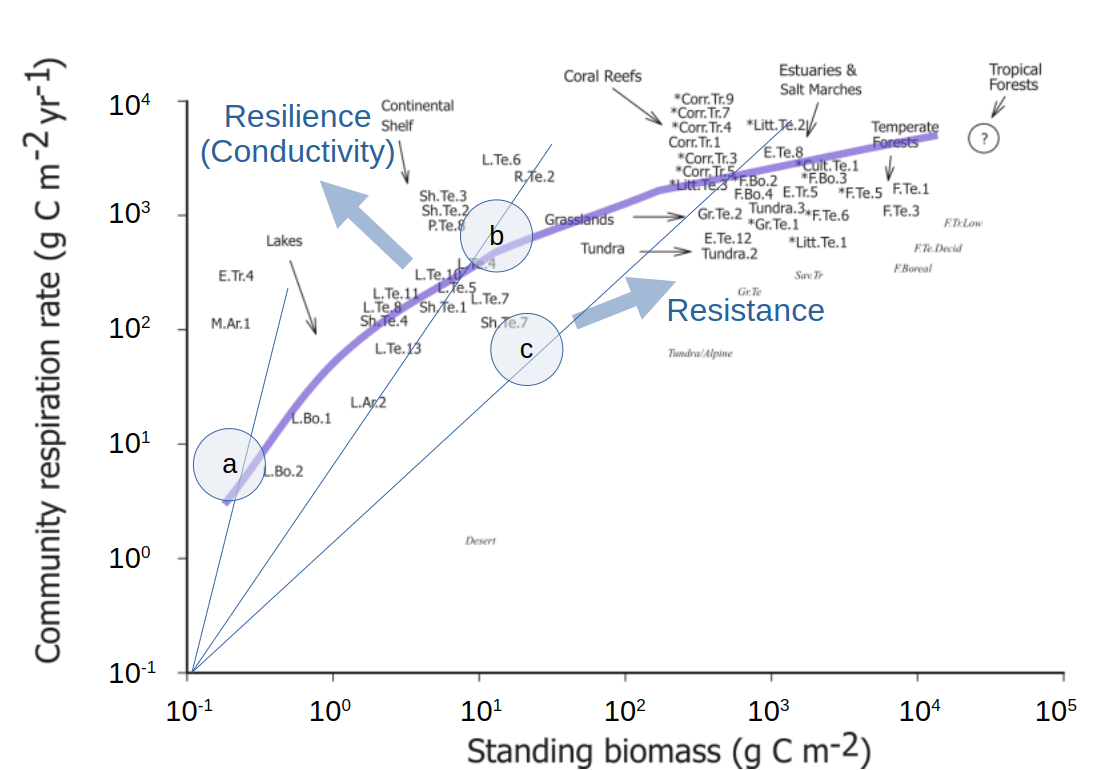
\includegraphics[width=0.8\textwidth,height=\textheight]{media/fig2.png}
\caption{The relationship between Respiration rate (a proxy for entropy
production) and biomass (a proxy for biovolume). Data were obtained from
the literature (see Choi 2002, Appendix 7). The form of this
relationship is constrained by allometric relationships between size and
metabolic rates. Due to this constraint, high ``resilience'' systems
(that is, high Respiration/Biomass ratios, eg. (a), or alternatively
high conductivity) are also generally lower resistance systems (low
biomass); and low resilience systems (low Respiration/Biomass ratios)
are also more resistant systems (high biomass), resistant in the sense
of the relative size of a perturbation (e.g.~system (b)). Any local
deviations from this pattern (e.g., c if perturbed from b) represents a
globally unstable situation and a return towards the global pattern
becomes more probable. Within each system, local deviations from the
system-specific expected behaviour represents a more ecologically
unstable situation. As such, ecologically (``local'') and evolutionarily
(``global'') favored directions for change can be antagonistic or
mutualistic, depending upon the specifics of the configuration of the
system concerned. NOTE: systems marked with an asterisk (\(*\))
represent order of magnitude estimates; italicized systems indicate the
relative magnitude of the Net primary production of representative
systems and so serves to approximately delineate a reasonable lower
bound of community respiration rates for each representative system
(respiration \textgreater\textgreater{} production). The codes are
structured as follows: {[}ecological type{]}.{[}climatic region{]}.{[}ID
number{]}. Climatic regions: Te=temperate; Tr=tropical; Ar=arctic;
Bo=boreal. Ecological types: E=estuary/brackish water; L=whole lake;
P=freshwater pelagic; Lit=littoral; M=marine pelagic; Sh=continental
shelf; CR=coral reef; R=river; Tu=tundra; Gr=grassland; Cul=culture; and
F=forest. \label{fig_lsd}}
\end{figure}

In the \emph{intensive} approach, there is an explicit expectation of
local \emph{Conjugate effects} (i.e., local ``steady-states'' or local
``homeostasis''; Fig. \ref{fig_lsd}). At an organismal level, this
expectation of homeostasis is not usually considered surprising by the
medical and organismal health literature as it is a necessary constraint
for the continuity of life. However, at the population, ecological,
evolutionary or even planetary levels of organization/space-time scales,
arguments relating to homeostasis has usually been met with skepticism
and ridicule, and pejoratively labeled as ``vitalism'', ``Lamarckism'',
``Panglossianism'' or ``teleological'' (e.g., Tansley 1935, Gould and
Lewontin 1979, Dawkins 1986, Mayr 1991, Grimm and Wissel 1997). The
importance, in this context, is that this thermodynamic principle
provides a local directionality of change that is clear and consistent
from organismal to sub-cellular to earth-system scales, without
resorting to teleology -- an expectation that is based upon, simply the
directionality of time; and potentially independent of the macroscopic
\emph{extensive} thermodynamic variables/processes.

This is a very significant contribution to ecology as prior to Onsager
and Prigogine, macroscopic thermodynamics only gave an indication that
entropy of the universe increased monotonically, free energy gradients
tend to dissipate and microscopic disorder would increase. Prigogine
(1955) and Prigogine et al.~(1972) used the term, ``dissipative
structures'', to denote these (locally) structured flows of matter and
energy (reactions; \(dS^\ddagger_i\)) that results in low (local,
intensive)\(^2\) entropy by either producing less entropy and/or
``exporting'' it to the external environment, and so respecting the
overall expectations of the (macroscopic extrinsic) \emph{entropy} to
increase over time. In other words, life can borrow free energy from the
environment to create local order (\emph{(local order \(<=>\) local
order) \(\rightarrow\) (global disorder)}); exporting entropy to the
exterior. The interpretation is that these hierarchical \emph{cascades}
of dissipative structures (Fig. \ref{fig_cascade}, area (C); Choi and
Patten 2001, O'Neill et al.~1986) represent \emph{local} departures
(fluctuations) from steady states, across multiple scales, such that
they operate in a manner analogous to the cascade of energy in turbulent
phenomena (Kolmogorov 1941), while still respecting the macroscopic
propensity of the \(2^{nd}\) law. Again, there is nothing controversial
here, and that is exactly the point. The exception being that
directionality now does not simply follow empirical patterns but rather,
there may be a thermodynamic basis for the expectations and
observations.

Some of the expectations of the ``least \emph{specific} dissipation of
energy'' have been examined and suggested to be related to overall
size-structure of ecosystems. They lead to a simple and unambiguous way
of measuring ecosystem-level fluctuations (perhaps better called,
``perturbation spectra''; Choi et al.~1999). The study of
\emph{intensive} thermodynamic processes in ecosystems shows much
promise due to their strong connections with the ideas of stability and
integrity in systems that are the product of numerous processes,
spanning large ranges in space, time and organisational scales (Choi and
Patten 2001).

A particularly promising and interesting connection that is worth noting
is the relationship of \(L\) to the \emph{community matrix} of
multi-species interactions in ecology (Yodzis 1981, Michaelian 2005). If
the latter are expressed as (local, intensive)\(^2\) entropy production
per unit biomass or number (i.e., in units of a ``phenomenological
force''), relative to a reference state (biomass or numerical density
centered to their respective means), then they can behave as
``conductivities'' in Onsager relations: we may expect reciprocity
relations between species if their relationships are causal and not
spurious! Some will be weak and others strong. The question becomes:
What conditions permit these \emph{Conjugate effects} to increase or
decrease/strengthen/weaken? What conditions make these \emph{Conjugate
effects} alter completely and new relations and new transport processes
to be established? In other words, this is evolution: selection and
adaptation, genetic and phenotypic plasticity, expressed in terms of
specific entropy production!

For example, if the contributions to (local intrinsic) specific
dissipation of one species is changed (due to external perturbation or
say human exploitation, habitat loss, rapid climate change, etc), the
biomass (or biovolume) of another reciprocal species will also change to
compensate (\emph{Conjugate effects}). Further, if we recall that
specific dissipation is proportional to mass specific metabolic rates
(e.g., see, Kleiber 1947, Bertalanffy 1950, Choi et al.~1999, Choi and
Patten 2001, Fath et al.~2001) then we can understand that this means,
increasing the abundance of one component (e.g., a predator) can have an
effect upon the specific metabolic rate of a prey (or competitor for
that matter). This might seem matter of fact and not too surprising. But
the reciprocal nature of these relations near a local steady state also
suggest that altering the specific rate of a prey can have an inverse
influence on that of the predator (or competitor). Sometimes correlation
can mean causation!

Ultimately, specific metabolism is, due to the allometry of metabolism,
closely related to size. So this simple relationship can be interpreted
as: altering the size structure of a predator can alter the size
structure of a prey, and vice versa, especially so if both are near
their respective stable size structures. This is not a controversial
statement. It also suggests that if total system biomass is constrained
to be constant, then total system metabolism will instead respond or
that if total metabolism is constrained then biomass will respond. If
both biomass and metabolic rate are constrained then other biochemical
processes (efficiency, adaptation) are expected to respond, suggesting
expectations in terms of evolutionary change and even speciation events.
That is local biodiversity expectations can change, simply due to these
energetic processes. Fascinating and testable expectations, that in
hindsight seem obvious and unsurprising, except that they derive from a
consideration of Onsager's relations.

Other potential applications are found in Oster et al.~(1971) for
electrodynamics, Prigogine et al.~(1972) for chemical dynamics,
Mikulecky (1985) on cell membrane dynamics. Further, attempts were made
to extend the Lyapunov stability analysis into the nonlinear realm using
variational principles by Nicolis and Prigogine (1989) and many others.
Not surprisingly, there are no guarantees that universal stability
criteria exist in nonlinear systems; they tend to have complex stability
regimes or \emph{attractors} (Byers and Hansell 1996, Shiner and
Sieniutycz 1994). Interestingly, Crooks (1999) and England (2013)
suggest some statistical generalizations may still be possible in highly
non-equilibrium conditions, as entropy production can be linked to
Markov transition probabilities in a statistical-fluctuation process
representation of biochemical reactions (i.e., in an
information-theoretic sense). But again, we would need a strong or at
least believable probabilistic ecological model before a similar type of
approach can be attempted to describe ecological dynamics. Odum and
Pinkerton (1955) tried to generalize from Onsager's relations to make
statements on thermodynamic efficiencies after noting the quadratic form
of the resultant total power output as a function of efficiencies. The
presence of these power maxima were suggested to substantiate Lotka's
(1922) heuristic arguments for the expectation of maximum total power
throughput in systems operating under Darwinian selection (akin to
Prigogine's \emph{Order through fluctuation} scenario; see Choi and
Patton 2001). They, however, did not account for the action of
\emph{Conjugate effects} that adaptively balance and stabilize these
flows (Choi et al.~1999).

\section{Summary}\label{summary}

Thermodynamics continues to have a critical role to play in the future
evolution of the field of ecology. It provides a strong and systemic and
integrative foundation and scaffolding. In the ecological context, we
are now perhaps still at a stage similar to when Carnot began measuring
efficiencies. We have the benefit of their experiences and that of
Boltzmann and Onsager. There is much to do and a great richness to be
expected as a deeper appreciation of thermodynamic constraints,
especially those of Onsager, develops and guides us to construct more
integrated ecological concepts and models. Currently, most authors seem
to be completely unaware of the rather significant contributions of
Onsager and Prigogine. We hope this review will inspire the next
generation of scientists to help us consolidate a field that is in great
need of an integrative foundation and vision.

\section{References}\label{references}

Aoki, I. (1989). Entropy flow and entropy production in the human body
in basal conditions. \emph{Journal of theoretical Biology}, 141,
pp.11-21.

Aoki, I. (1993). Inclusive Kullback index -- a macroscopic measure in
ecological systems. \emph{Ecological Modelling}, 66, pp.289-299.

Aoki, I. (1995). Entropy production in living systems: from organisms to
ecosystems. \emph{Thermochimica Acta}, 250, pp.359-370.

Babloyantz, A. 1986. Molecules, Dynamics and Life: An introduction to
Self-Organization of Matter. Wiley-InterScience, Toronto.

Bell, G., 1982. The Masterpiece of Nature: The Evolution and Genetics of
Sexuality. Croom Helm Ltd.~

Bertalanffy, L. von. (1950). The theory of open systems in physics and
biology. \emph{Science}, 111, pp.23-29.

Briedis, D. and Seagrave, R.C. (1984). Energy transformation and entropy
production in living systems I. Applications to embryonic growth.
\emph{Journal of theoretical Biology}, 110, pp.173-193.

Byers, R.E. and Hansell, R.I.C. (1996). Implications of semi-stable
attractors for ecological modelling. \emph{Ecological Modelling}
89:59-65.

Carnot, S. (1824). \emph{Reflexions sur la puissance motrice du feu}.
Bachelier, Paris. (English translation in R. Fox. 1986. \emph{Reflexions
on the motive power of fire}. Manchester University Press.)

Carathéodory, C. (1909). Untersuchung über die Grundlagen der
Thermodynamik, \emph{Math. Annalen}, 67, pp.355-386.

Chakrabarti, C.G. and Ghosh, K., 2009. Non-equilibrium thermodynamics of
ecosystems: Entropic analysis of stability and diversity. Ecological
Modelling, 220, pp.1950-1956.

Chapman, E.J., Childers, D.L., Vallino, J.J. (2016). How the Second Law
of Thermodynamics Has Informed Ecosystem Ecology through Its History.
\emph{BioScience}, 66, pp.27-39.

Clausius, R. (1850). Uber die bewegende Kraft der Wärme und die Gesetze,
welche sïch daraus für die Wärmelehre selbst ableiten lassen.
\emph{Annalen der Physik Und Chemie}, 79, pp.368-397. (English
translation in J. Kestin. 1976. \emph{Second Law of Thermodynamics},
John Wiley \& Sons Inc.~346 p.)

Choi, J.S., 2019. Thermodynamics in Ecology. In: Fath, B.D. (ed),
Encyclopedia of Ecology, 2nd edition, vol.~1, pp.~653--662. Oxford:
Elsevier.

Choi, J.S., Mazumder, A. and Hansell, R.I.C. (1999). Measuring
perturbation in a complicated, thermodynamic world. \emph{Ecological
Modelling}, 117, pp.143-158.

Choi, J.S. and Patten, B.C. (2001). Sustainable development: lessons
from the paradox of enrichment. \emph{Ecosystem Health}, 7:163-178.

Crooks, G.E. (1999). Entropy production fluctuation theorem and the
nonequilibrium work relation for free energy differences. Physical
Review E, 60, pp.2721-2726.

Dawkins, R. (1986). \emph{The blind watchmaker: Why the evidence of
evolution reveals a universe without design}. WW Norton \& Company.

Dewar, R.C. and Porté, A., 2008. Statistical mechanics unifies different
ecological patterns. Journal of theoretical biology, 251, pp.389-403.

Dewar, R.C., 2010. Maximum entropy production and plant optimization
theories. Philosophical Transactions of the Royal Society of London B:
Biological Sciences, 365, pp.1429-1435.

Eigen, M., and Schuster, P. (1979). \emph{The hypercycle: a principle of
natural self-organization}. Springer-Verlag, New York.

Elith, J., Phillips, S.J., Hastie, T., Dudík, M., Chee, Y.E. and Yates,
C.J. (2011). A statistical explanation of MaxEnt for ecologists.
\emph{Diversity and distributions}, 17, pp.43-57.

Elton, C. (1927). \emph{Animal Ecology}. Sidgwick and Jackson, London.

England, J.L. (2013). Statistical physics of self-replication. The
Journal of chemical physics, 139, pp.121923(1-8).

Eppley, R. and Peterson, B. (1967). Particulate organic matter flux and
planktonic new production in the deep ocean. \emph{Nature}, 182,
pp.677-682.

Fath, B.D., Patten, B.C. and Choi, J.S. (2001). Complementarity of
ecological goal functions. \emph{Journal of theoretical biology}, 208,
pp.493-506.

Fath, B.D., Jørgensen, S.E., Patten, B.C. and Straškraba, M. (2004).
Ecosystem growth and development. \emph{Biosystems}, 77, pp.213-228.

Gibbs, J. W. (1902). \emph{Elementary Principles in Statistical
Mechanics, developed with especial reference to the rational foundation
of thermodynamics}. Charles Scribner's Sons., New York.

Gladyshev, G.P. (1978). On the thermodynamics of biological evolution.
\emph{Journal of theoretical Biology} 75, pp.425-441.

Glansdorff, P., Nicolis, G. and Prigogine, I. (1974). The Thermodynamic
Stability Theory of Non-Equilibrium States. \emph{Proceedings of the
National Academy of Science USA}, 71, pp.197-199.

Gould, S.J. and Lewontin, R.C. (1979). The spandrels of San Marco and
the Panglossian paradigm: a critique of the adaptationist programme.
\emph{Proceedings of the Royal Society of London, Series B: Biological
Sciences}, 205, pp.581-598.

Grimm, V. and Wissel, C. (1997). Babel, or the ecological stability
discussions: an inventory and analysis of terminology and a guide for
avoiding confusion. \emph{Oecologia}, 109, pp.323-334.

Gündüz, Ö. and Gündüz, G. (2014). The phase space interpretation of the
Le Chatelier‐Braun principle and its generalization as a principle of
natural philosophy. Physics Essays. 27. 10.4006/0836-1398-27.3.404.

Halbach, U., 1973. Life table data and population dynamics of the
rotifer, Bracionuc calyciflorus pallas as influenced by periodically
oscillating temperature. In: Wieser, W. (Ed.), Effects of Temperature on
Ectothermic Organisms: Ecological Implications and Mechanisms of
Compensation. Springer-Verlag, New York, pp.~217--228.

Holdaway, R.J., Sparrow, A.D. and Coomes, D.A., 2010. Trends in entropy
production during ecosystem development in the Amazon Basin.
Philosophical Transactions of the Royal Society of London B: Biological
Sciences, 365, pp.1437-1447.

Hutchinson G.E. (1959). Homage to Santa Rosalia, or why are there so
many kinds of animals. \emph{American Naturalist} 93, pp.145--159.

Jaynes, E.T. (1957). Information theory and statistical mechanics.
\emph{Physical review}, 106, pp.620-630.

Johnson, L. (1981). The thermodynamic origin of ecosystems.
\emph{Canadian Journal of Fisheries and Aquatic Science} 38:571-590.

Jørgensen, S.E., Nielsen, S.N. and Mejer, H. (1995). Emergy, environ,
exergy and ecological modelling. \emph{Ecological modelling}, 77,
pp.99-109.

Jørgensen, S.E., 2012. Integration of Ecosystem Theories: A Pattern
(Vol. 3). Springer Science \& Business Media.

Kay, J.J. (1991). A Non-equilibrium Thermodynamic Framework for
Discussing Ecosystem Integrity. \emph{Environmental Management}, 15,
pp.483--495.

Kleiber, M. (1947). Body size and metabolic rate. Physiological Reviews,
27, pp.511--541.

Kleidon, A., 2010. A basic introduction to the thermodynamics of the
Earth system far from equilibrium and maximum entropy production.
Philosophical Transactions of the Royal Society of London B: Biological
Sciences, 365, pp.1303-1315.

Kolmogorov, A.N. (1941). Local structure of turbulence in an
incompressible fluid for very large Reynolds numbers. \emph{Doklady
Academy of Science USSR}, 31, pp.301-305.

Landsberg, P.T. (1972). The Fourth Law of Thermodynamics. \emph{Nature},
238, pp.299-231.

Lieb, E.H., and Yngvason, J. (1999). The Physics and mathematics of the
Second law of Thermodynamics. \emph{Physics Reports}, 310, pp.1-96.

Lindeman, R.L. (1942). The trophic-dynamic aspect of ecology.
\emph{Ecology}, 23, pp.399--418.

Lotka, A.J. (1922). Contribution to the energetics of evolution.
\emph{Proceedings of the National Academy of Science USA}, 8,
pp.147-151.

Lovelock, J.E. (1972). Gaia as seen through the atmosphere.
\emph{Atmospheric Environment}, 6, pp.579--580.

Lovelock, J.E. and Margulis, L. (1974). Atmospheric homeostasis by and
for the biosphere: the Gaia hypothesis. \emph{Tellus, Series A.
Stockholm: International Meteorological Institute}, 26, pp.2--10.

Lurié, D., and Wagensberg, J. (1979). Non-equilibrium thermodynamics and
biological growth and development. \emph{Journal of theoretical
Biology}, 78, pp.241-250.

MacArthur, R.H. and Pianka, E.R. (1966). On the optimal use of a patchy
environment. \emph{American Naturalist}, 100, pp.603--609.

Mann, K.H. (1972). Ecological energetics of the seaweed zone in a marine
bay of the Atlantic Coast of Canada. I. Zonation and biomass of
seaweeds. \emph{Marine Biology}, 12, pp.1-10.

Margalef, R. (1963). On certain unifying principles in ecology.
\emph{The American Naturalist}, 898, pp.357-374.

Martyushev, L.M., 2010. The maximum entropy production principle: two
basic questions. Philosophical Transactions of the Royal Society of
London B: Biological Sciences, 365, pp.1333-1334.

Mazur, P. 1997. Onsager's Reciprocal Relations and Thermodynamics of
Irreversible Processes. Periodica Polytechnica Ser. Chem. Eng. 41:
197-204.

Matsuno, K. (1978). Evolution of dissipative systems: a theoretical
basis for Margalef\textquotesingle s principle of ecosystems.
\emph{Journal of Theoretical Biology,} 70, pp.23-31.

Mayr, E. (1991). The ideological resistance to Darwin\textquotesingle s
theory of natural selection. \emph{Proceedings of the American
Philosophical Society}, 135, pp.123-139.

Meysman, F.J. and Bruers, S., 2010. Ecosystem functioning and maximum
entropy production: a quantitative test of hypotheses. Philosophical
Transactions of the Royal Society of London B: Biological Sciences, 365,
pp.1405-1416.

Michaelian, K., 2005. Thermodynamic stability of ecosystems. Journal of
theoretical biology, 237, pp.323-335.

Mikulecky, D.C. (1985). Network thermodynamics in biology and ecology:
an introduction. In: R.E. Ulanowicz and T. Platt (eds.), Ecosystem
theory for biological oceanography. \emph{Canadian Bulletin of Fisheries
and Aquatic Sciences}, 213, pp.163-175.

Miller, D.G. 1959. Thermodynamics of Irreversible Processes, The
experimental verification of the Onsager Reciprocal Relations. Chemical
Reviews, 16-37.

Meixner, J. (1973). The entropy problem in thermodynamics of processes.
\emph{Rheologica Acta}, 12, pp.465--467.

Müller, F. (1998). Gradients in ecological systems. \emph{Ecological
Modelling}, 108, pp.3-21.

Nicolis, G. and Prigogine, I. (1977). \emph{Self-Organization in
Non-Equilibrium Systems}. Wiley.

Nicolis, G. and Prigogine, I. (1989). \emph{Exploring complexity: An
introduction}. WH Freeman.

Odum, E.P. (1969). The strategy of ecosystem development.
\emph{Science}, 164, pp.262-270.

Odum, H.T. (1996). \emph{Environmental Accounting: Emergy and Decision
Making}. John Wiley, NY. 370 p.~

Odum, H.T. and Pinkerton, R.C. (1955). Time's speed regulator: the
optimum efficiency for maximum power output in physical and biological
systems. \emph{American Scientist}, 43, pp.321-343.

O'Neill, R.V., DeAngelis, D.L., Waide J.B. and Allen, T.F.H. (1986). A
Hierarchical Concept of Ecosystems. \emph{Monographs in population
biology}. Princeton University Press. 253p.

Onsager, L. (1931a). Reciprocal Relations in Irreversible Processes. I.,
\emph{Physical Review}, 37, pp.405--426.

Onsager, L. (1931b). Reciprocal Relations in Irreversible Processes.
II., \emph{Physical Review}, 38, pp.2265-2279.

Onsager, L. and Machlup, S. 1953. Fluctuations and irreversible
processes, \emph{Physical Review}, 91, 1505--1512.

Oster, G., Perelson, A. and Katchalsky, A. (1971). Network
thermodynamics. \emph{Nature} 234, pp.393-399.

Öttinger, H. C., Peletier, M. A., and Montefusco, A. 2021. J.
Non-Equilibrium Thermodynamics 46:1-13.

Patten, B.C. (1978). Systems approach to the concept of environment.
\emph{Ohio Journal of Science}, 78, pp.206-222.

Peters, R.H. (1991). A critique for ecology. Cambridge University Press,
New York.

Planck, M. (1901). Ueber das Gesetz der Energieverteilung im
Normalspectrum. \emph{Annalen der Physik}, 4, pp.553-563.
(\href{https://web.archive.org/web/20081217042934/http://dbhs.wvusd.k12.ca.us/webdocs/Chem-History/Planck-1901/Planck-1901.html}{English
translation})

Prigogine, I. (1955). \emph{Thermodynamics of irreversible processes}.
John Wiley and Sons, New York. 147 p.~

Prigogine, I., Nicolis, G. and Babloyantz, A. (1972). Thermodynamics of
evolution. \emph{Physics today}, 25, p.23.

Regier, H.A. and Kay, J.J. (1996). An heuristic model of transformations
of the aquatic ecosystems of the Great Lakes-St.~Lawrence River Basin.
\emph{Journal of Aquatic Ecosystem Stress and Recovery} (Formerly
\emph{Journal of Aquatic Ecosystem Health}), 5, pp.3-21.

Russell, F.L., Zippin, D.B., Fowler, N.L. 2001. Effects of White-tailed
Deer (Odocoileus virginianus) on Plants, Plant Populations and
Communities: A Review. \emph{The American Midland Naturalist},
Jul;146(1): 1--26.

Schneider, E.D. and Kay, J.J. (1994). Life as a manifestation of the
second law of thermodynamics. \emph{Mathematical and computer
modelling}, 19, pp.25-48.

Schneider, E.D. and Sagan, D. (2005). \emph{Into the cool: Energy flow,
thermodynamics, and life}. University of Chicago Press.

Schrödinger, E. (1944). \emph{What Is Life? The Physical Aspect of the
Living Cell.} Cambridge University Press, Cambridge.

Shannon, C.E. (1948). A Mathematical Theory of Communication. \emph{Bell
System Technical Journal}, 27, pp.379--423.

Shiner, J.S and Sieniutycz, S. 1994. The Chemical Dynamics of Biological
Systems: Variational and Extremal Formulations. Prog. Biophys. molec.
Biol. 62:203-221.

Smith, R.S., Bloomfield, S.F., Rook, G.A. 2012. The Hygiene Hypothesis
and its implications for home hygiene, lifestyle and public health. Home
Hygiene \& Health. Best Practice, Review. 14/12/2012. IFH.

Strachan, D. 2000. Family Size, Infection and Atopy: The First Decade of
the `Hygiene Hypothesis.' Thorax 55 (90001): 2S -- 10.
https://doi.org/10.1136/thorax.55.suppl\_1.S2.

Wiley, E.O. and Brooks, D.R. (1982). Victims of history -- a
nonequilibrium approach to evolution. \emph{Systematic Biology}, 31,
pp.1-24.

Tansley, A.G. (1935). The use and abuse of vegetational terms and
concepts. \emph{Ecology}, 16, pp.284--307.

Thomson, W. (Lord Kelvin). (1849). An account of Carnot's theory of the
motive power of heat; with numerical results deduced from Regnault's
experiments on steam, \emph{Transactions of the Royal Society of
Edinburgh}, 16, pp.541-574.

Ulanowicz, R.E. and Hannon, B.M. (1987). Life and the Production of
Entropy. \emph{Proceedings of the Royal Society of London Series B},
232, pp.181-192.

Ulanowicz, R.E., Jørgensen, S.E. and Fath, B.D. (2006). Exergy,
information and aggradation: An ecosystems reconciliation.
\emph{Ecological Modelling}, 198, pp.520-524.

Vanriel, P. and Johnson, L. (1995). Action principles as determinants of
ecosystem structure: the autonomous lake as a reference system.
\emph{Ecology}, 76, pp.1741-1757.

van Valen, L. (1976). A new evolutionary law. \emph{Evolutionary
Theory}, 1, pp.1-30.

Verhás J. (2014). Gyarmati's Variational Principle of Dissipative
Processes. \emph{Entropy}. ; 16(4):2362-2383.
https://doi.org/10.3390/e16042362

Washida, T. (1995). Ecosystem configurations consequent on the maximum
respiration hypothesis. \emph{Ecological Modelling}, 78, pp.173-193.

Watson, A.J. and Lovelock, J.E. (1983). Biological homeostasis of the
global environment: the parable of Daisyworld. Tellus B. 35: 286--9.

Whittaker, R. H. (1953). A consideration of climax theory: the climax as
a population and pattern. \emph{Ecological Monographs}, 23:41-78.

Wicken, J.S. (1980). A thermodynamic theory of evolution. \emph{Journal
of theoretical Biology}, 87, pp.9-23.

Yen, J.D.L., Paganin, D.M., Thomson, J.R. and MacNally, R. (2014).
Thermodynamic extremization principles and their relevance to ecology.
\emph{Austral Ecology}, 39, pp.619--632.

Yodzis, P. (1981). The stability of real ecosystems. \emph{Nature},
289:674-676.

Yodzis, P. (1988). The Indeterminacy of Ecological Interactions as
Perceived Through Perturbation Experiments. \emph{Ecology},
\emph{69}(2), 508--515. https://doi.org/10.2307/1940449

Zotin, A.I. and Zotina, R.S. (1967). Thermodynamics aspects of
developmental biology. \emph{Journal of theoretical Biology} 17:57-75.

\begin{verbatim}
\end{verbatim}





 
%% The Appendices part is started with the command \appendix;
%% appendix sections are then done as normal sections
%% \appendix

%% \section{}
%% \label{}

%% References
%%
%% Following citation commands can be used in the body text:
%% Usage of \cite is as follows:
%%   \cite{key}          ==>>  [#]
%%   \cite[chap. 2]{key} ==>>  [#, chap. 2]
%%   \citet{key}         ==>>  Author [#]

%% References with bibTeX database:

 

\printbibliography






%%%%%%%%%%%%%%%%%%%%%%%%%%%%%%%%%%%%%%%%%%%%%%%%%%%%%%%%%%%%
%%% SUPPLEMENTARY MATERIAL / APPENDICES
%%%%%%%%%%%%%%%%%%%%%%%%%%%%%%%%%%%%%%%%%%%%%%%%%%%%%%%%%%%%

% 
%%%%%%%%%%%%%%%%%%%%%%%%%%%%%%%%%%%%%%%%%%%%%%%%%%%%%%%%%%%%
%%% ARTICLE END
%%%%%%%%%%%%%%%%%%%%%%%%%%%%%%%%%%%%%%%%%%%%%%%%%%%%%%%%%%%%

%  

% % \end{CSLReferences}

\end{document}
% \endinput
